% !TEX encoding = UTF-8
% !TEX TS-program = pdflatex
% !TEX root = ../main.tex
% !TEX spellcheck = en-EN

%************************************************
% Parlare dei dataset utilizzati
% parlare di come sono stati raccolti i dati del dataset nostro
% parlare della data augmentation
% parlare dei primi risultati ottenuti
% parlare delle metriche che sono state usate con i corrispettivi risultati

In plant phenotyping, several datasets were used, one being the Multi-Modality Imagery Database for Plant Phenotyping, and the
Komatsuna dataset. these two datasets were chosen for leaf variety and type. Both have similar "broad" leaves. To get the most out of neural networks we tested and
adapted our datasets to the most famous dataset used in object detection and image segmentation, COCO. To do this we used coco annotator \cite{cocoannotator}, where through
a script written by us we have adapted the annotations within the dataset in COCO format, and once imported into the annotator, we have finished and fixed the masks.
This allowed us to make our dataset common to all the networks used so that we could compare the results obtained for both YOLACT and SOLO and Blendmask.
In this chapter, we will describe what are the datasets used and show how we used them and the results obtained

\section{Datasets}
\subsection{Multi-Modality Imagery Database}
Multi-Modality Imagery Database is provided by Michigan State University. It contains two different types of plants, that of the bean and Arabidopsis thaliana.
The images were taken at different times of the day at regular intervals. Regarding Arabidopsis the dataset is composed of a total of 2160 acquisitions with only
576 annotated images with a size of $116\times 119$, each acquisition is composed of four images one RGB, one depth, one infrared and one fluorescence. The bean
images instead is composed of 325 images of which 175 annotated with a dimension of $481\times 491$, but unlike the bean as annotated images are reported only those
fluorescent, then they will be inserted these within the network for training.

\begin{figure}[ht] 
    \centering
    \begin{subfigure}{.5\textwidth}
      \centering
      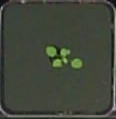
\includegraphics[width=.9\linewidth]{arabidopsis}
      \caption{Arabidopsis image from MMI database}
      \label{fig:sub1}
    \end{subfigure}%
    \begin{subfigure}{.5\textwidth}
      \centering
      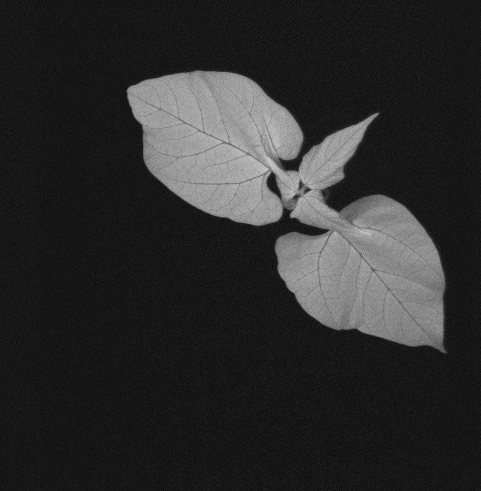
\includegraphics[width=.9\linewidth]{bean}
      \caption{Bean image from MMI database}
      \label{fig:sub2}
    \end{subfigure}
    \caption{Example of Multi-Modality Imagery Database images for training and validation}
    \label{fig:MMI}
\end{figure}

The total of the 751 images are divided into 2 sets with a split ratio of $60\%$ $40\%$, the training set with a total of 451 images and the validation set with a
total of 300 images. This can be performed by a script which randomly split the entire dataset into two or three sets and then recombine them into two or three files which
contains training, validation and optionally test set of images.

\subsection{Komatsuna Dataset}
Komatsuna, is a Japanese leaf vegetable, it belongs to the Brassica rapa family. This dataset consist of a 3d setup with two different kind of images. The 3D images are
divided into whole images containing the entire set of plants linked to a 3d image, these were collected on different days every four hours. These images, both RGB and
depth images, are $640\times 480$ in size, which will later be cropped according to what the network, in our solution, considers most appropriate. These images have been
placed at a distance of about 50cm from the plane, and have the following intrinsic matrix:

$$
\begin{pmatrix}
    382.641 & 0       & 223.248 \\     
    0       & 382.641 & 233.523 \\
    0       &       0 & 1
\end{pmatrix}
$$

We used these images as test images to validate the network trained specifically to recognize komatsuna leaves, and through the depth images and the intrinsic matrix
we sized the found leaves.

\begin{figure}[ht] 
  \centering
  \begin{subfigure}{.5\textwidth}
    \centering
    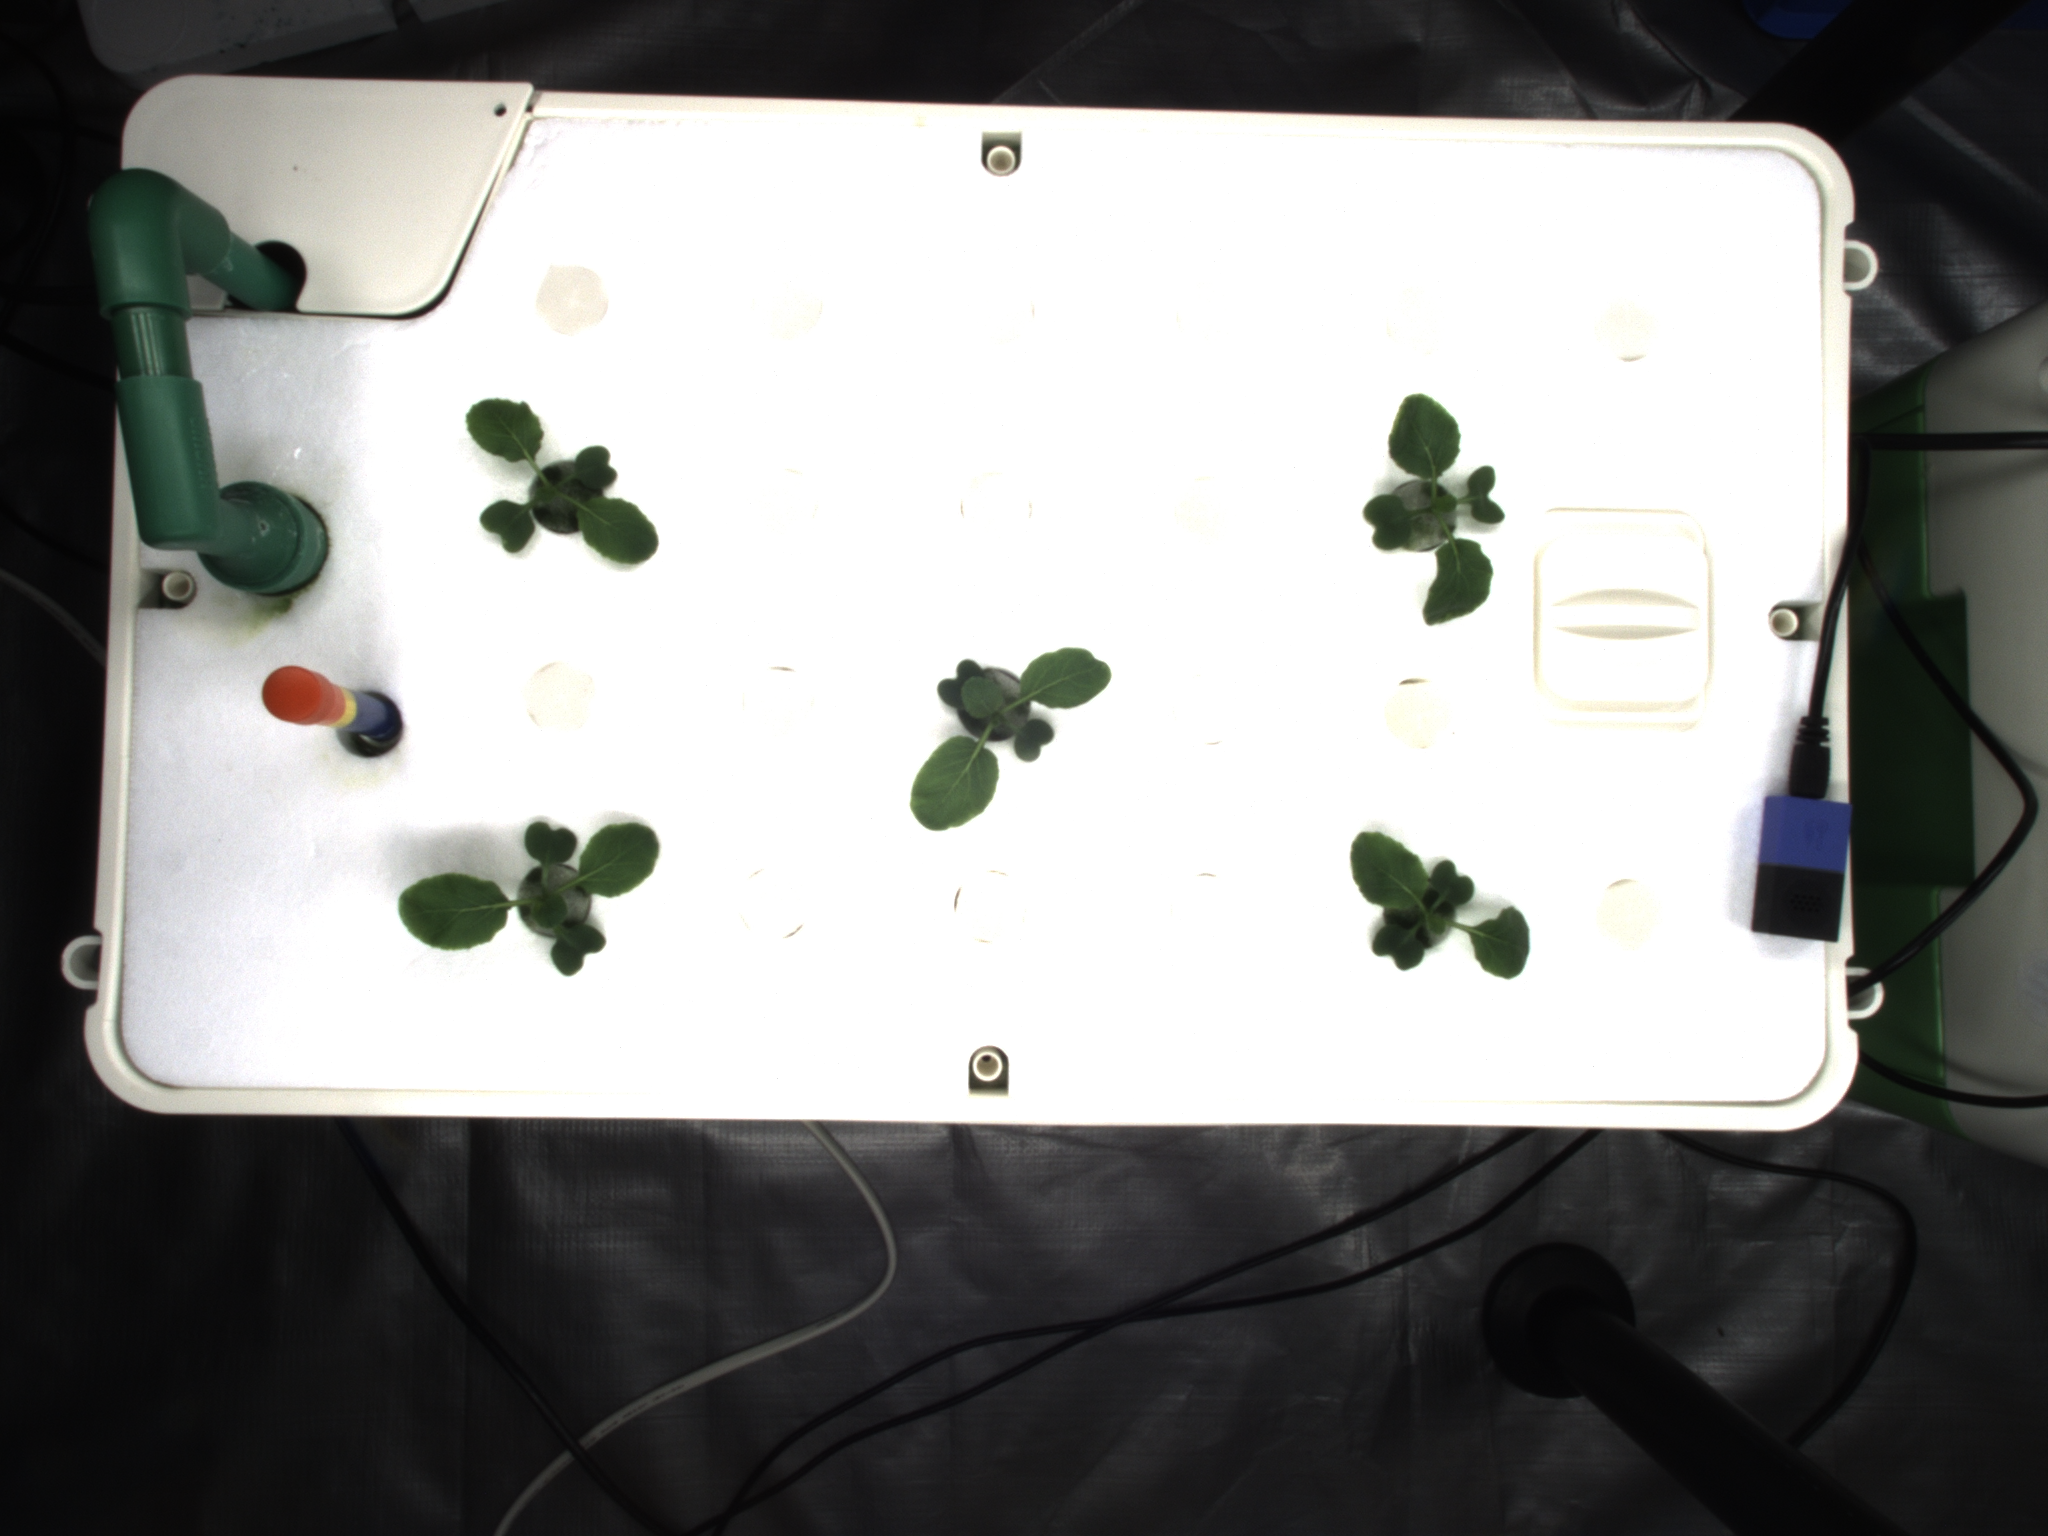
\includegraphics[width=.9\linewidth]{komatsuna_training}
    \caption{Training image for Komatsuna dataset}
    \label{fig:sub3}
  \end{subfigure}%
  \begin{subfigure}{.5\textwidth}
    \centering
    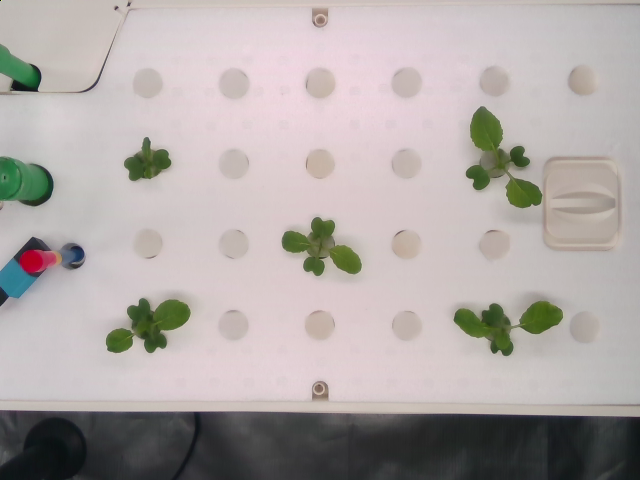
\includegraphics[width=.9\linewidth]{komatsuna_test}
    \caption{Test image for Komatsuna dataset}
    \label{fig:sub4}
  \end{subfigure}
  \caption{Komatsuna Dataset training, test images}
  \label{fig:komatsuna}
\end{figure}


The other images, concerning the multiview RGB, start from a higher dimension of $2048\times 1536$, without having the depth images. These have been divided plant by plant by
the authors obtaining a total of 900 images for the dataset with dimension $480\times480$. to improve even more the model obtained from the neural network we have increased
the dataset up to 4500 images, through the different techniques of rotation flip and blur, where we used 2700 images for training and 900 for validation, finally to test
the metrics we used the remaining 900 images.


\subsection{Our Dataset}
In our dataset we collect the most of images in a single day at a local farm, consisting of a set of images of basil seedlings. Some plants were subsequently collected
from which a second set of images was extrapolated over the next five days. The first set designed for training has a total of 128 images of size $640\times 480$
containing a total of 892 seedlings. 

\begin{figure}[ht] 
  \centering
  \begin{subfigure}{.5\textwidth}
    \centering
    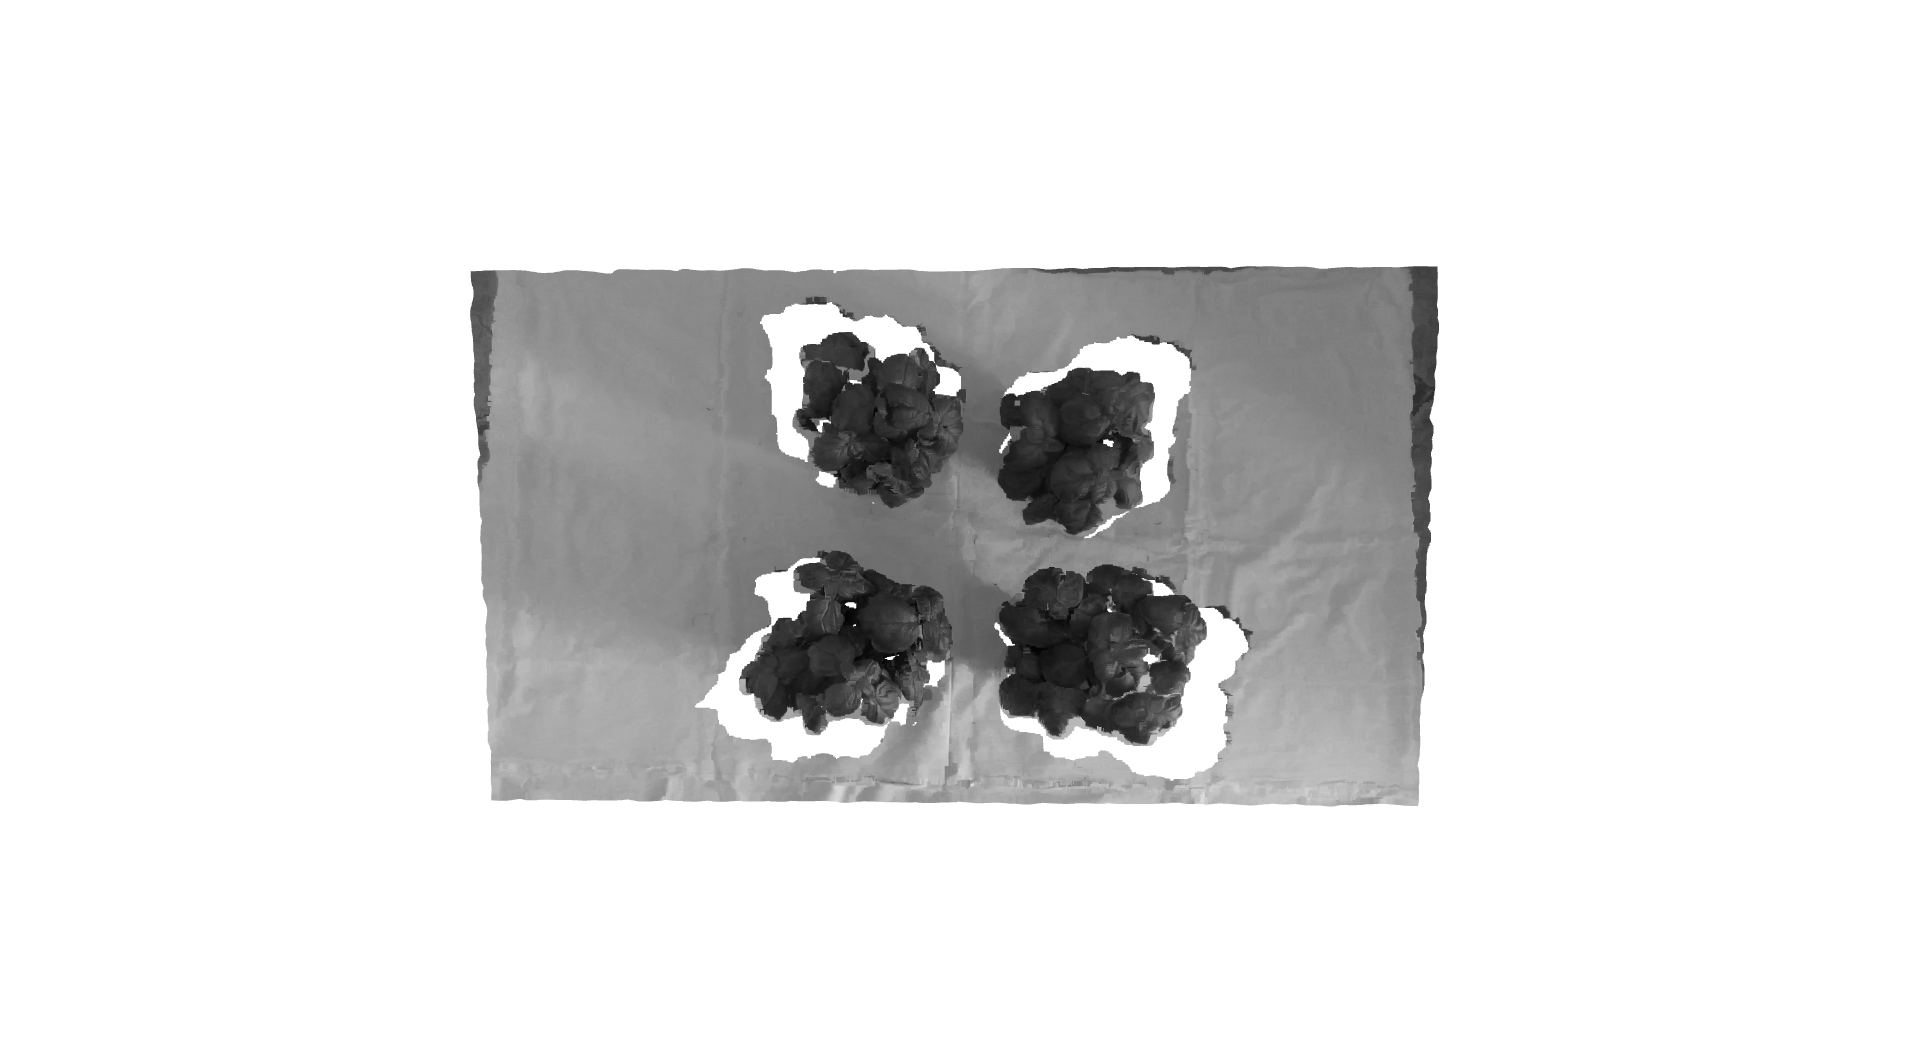
\includegraphics[width=.9\linewidth]{top_view}
    \caption{Top view of depth images}
  \end{subfigure}%
  \begin{subfigure}{.5\textwidth}
    \centering
    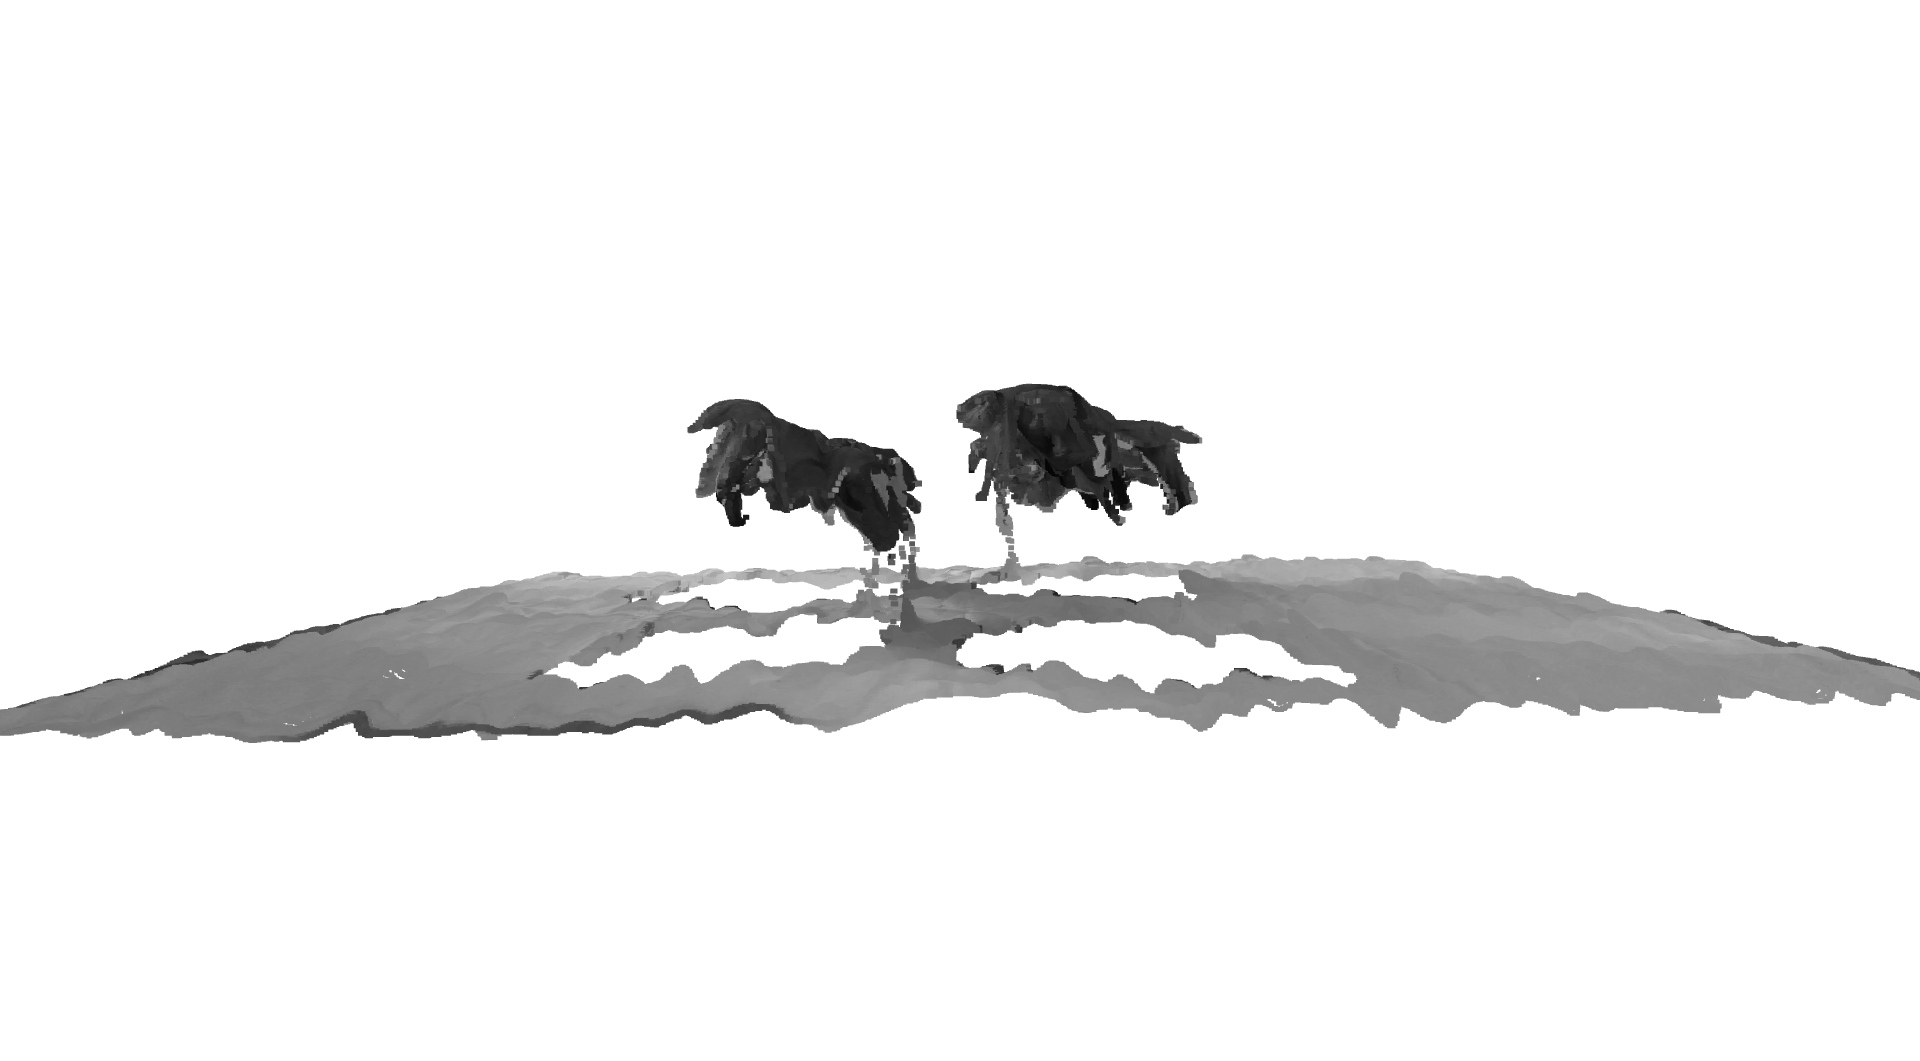
\includegraphics[width=.9\linewidth]{side_view}
    \caption{Side view of depth images}
  \end{subfigure}
  \caption{Example of depth images representation}
\end{figure}

All of these images have appropriately aligned depth images attached to them, so that 3D networks can also be trained. The second
set designed for testing consists of a set of images divided by days for a total of five days with 20 daily images. Their size is $1280\times 720$ with the depth images also
aligned. Each image consists of four seedlings rotated and swapped positions at each acquisition. On the last day, the dimensional information of the leaves that are
fully visible not covered by other leaves was also included.

\begin{figure}[ht] 
  \centering
  \begin{subfigure}{.5\textwidth}
    \centering
    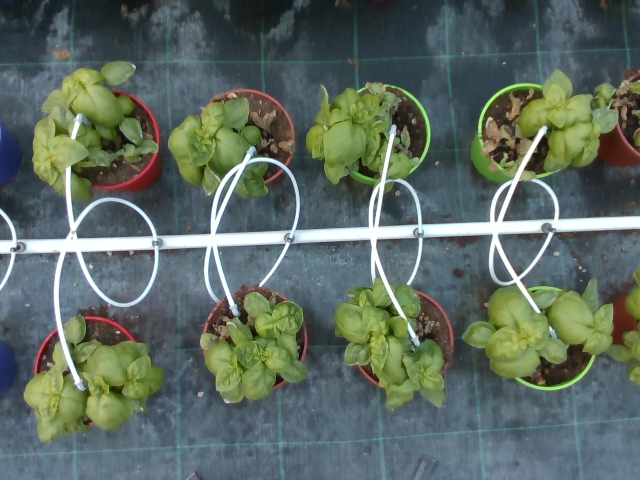
\includegraphics[width=.9\linewidth]{our_train}
    \caption{Training image for our dataset}
    \label{fig:sub5}
  \end{subfigure}%
  \begin{subfigure}{.5\textwidth}
    \centering
    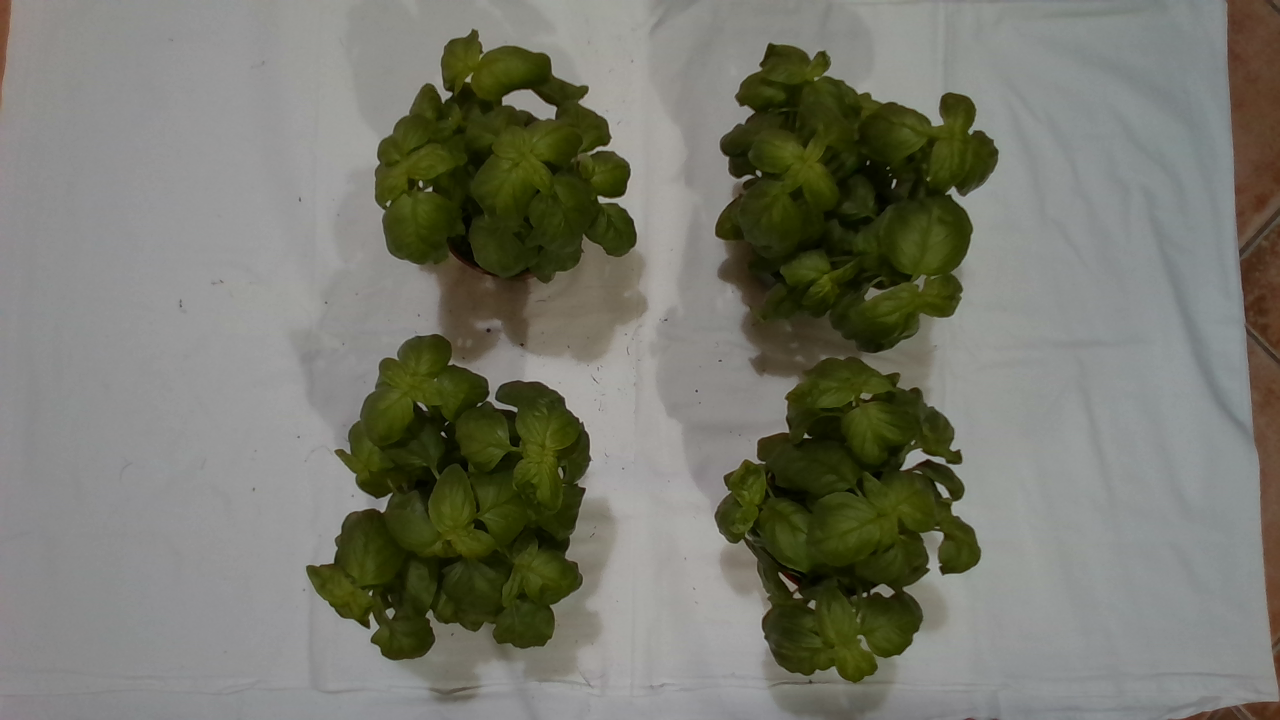
\includegraphics[width=.9\linewidth]{our_test}
    \caption{Test image for our dataset}
    \label{fig:sub6}
  \end{subfigure}
  \caption{Our Dataset training, test images}
  \label{fig:ourData}
\end{figure}

To be able then to do the dimensional calculation we made use of the intrinsic matrix provided by the camera used, an Intel RealSense D435:

$$
\begin{pmatrix}
    637.735 & 0       & 645.414 \\     
    0       & 637.735 & 349.205 \\
    0       &       0 & 1
\end{pmatrix}
$$

All images were acquired at a ground clearance of 92cm under varying but high light conditions. Placing a cloth in the background allowed us to adapt the network
trained via yolo for object detection to our dataset as well in order to automate the calculation of measurement validation.


\section{State of The art Comparison}
Several networks have been used, all of this are trained on a Nvidia 3090 with 24GB of dedicated RAM via the PyTorch framework, which is an efficient library for
building deep learning projects using the Python programming language. 



All of the nets are trained with both of the dataset Multi-Modality Imagery Database and Komatsuna, the first with both the images of Arabidopsis and Bean, 
but for practical reasons only fluorescence images are used for bean plants. The dataset has been divided into two parts: the train part is composed of 450
images, while the validation part used to calculate the metrics is composed of 300 images. The increased komatsuna has been divided into three parts train
validation and test where the first one consists of 2700 images and the other two of 900 images each. 

The first ones used are yolact and its variant yolact plus where, via ResNet-101 and ResNet-101 with deformed convolutions, they were trained with the two datasets.
Several attempts were made with various configurations but the most suitable turned out to be the ResNet-101 deformed and not, with a learning rate of $0.001$, were
also started several training sessions with different epochs but exceeded the hundred networks have not shown significant improvements.\\
Blendmask was trained only with the deformed ResNet-101 for both datasets with a learning rate of $0.001$ completing the training quickly with about 200 epochs,
increasing the number of the latter did not detect significant improvements.\\
The last one to be trained is SOLOv2, which was also tested with deformable convolutional networks on ResNet-101. After several tests we found a better performance
after about 200 epochs, on komatsuna with a learning rate of $0.001$, while for the images of the Multi-Modality Imagery Database, it was necessary to further lower
the learning rate of the network to $0.0001$ due to the smaller size of the images.


\subsection{Multi-Modality Imagery Database}
To validate our work we need to compare our results with what is the state of the art, thanks Bhugra, Garg, Chaudhury and Lall \cite{9411981}, we were able to establish that
the performance of the networks used are comparable to what is a more targeted solution like the one made by the authors of the paper.

\begin{figure}[h]
  \centering
  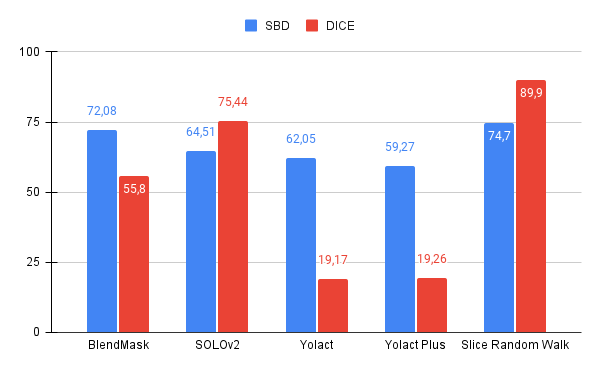
\includegraphics[width=.8\textwidth]{comparison_ppd}%
  \caption{Comparison between Blendmask\cite{chen2020blendmask}, SOLOv2\cite{wang2020solov2}, YOLACT\cite{bolya2019yolact} and \cite{9411981} on plant phenotyping dataset}%
\end{figure}

Thus, the proposed networks are able to perform realistically precise segmentations even on a varied dataset such as plant phenotyping.

\subsection{Komatsuna dataset}
With the previous results we can ascertain that the networks are able to behave in a similar way to what is a solution designed specifically for the problem at hand.
Then we compared what were the results obtained with komatsuna with what is the plant phenotyping dataset obtained from \cite{9411981}. 

\begin{figure}[ht]
  \centering
  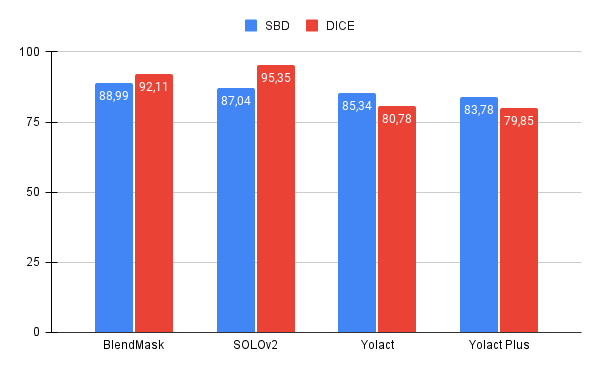
\includegraphics[width=.8\textwidth]{comparison_komatsuna}%
  \caption{Comparison between Blendmask\cite{chen2020blendmask}, SOLOv2\cite{wang2020solov2}, YOLACT\cite{bolya2019yolact}}%
\end{figure}

We have noticed that for komatsuna, also because of the higher quantity of images available, the results are much better and therefore able to extrapolate in
a more optimal way the leaves.

\subsection{Our Dataset}
To validate all the data we need to check whether the results obtained from the networks are valid or not. To do this we used our dataset where at first we
applied the yolo-net so as to obtain the individual images then through blendmask, we extrapolated the individual instances of the leaves.
We used Blendmask because even though SOLOv2 performed better on paper, it turned out in reality to be poorly adapted to a leaf type it had not seen before.
In fact Blendmask identified basil leaves better than SOLOv2, despite both being trained for komatsuna.

\begin{figure}[ht]
  \centering
  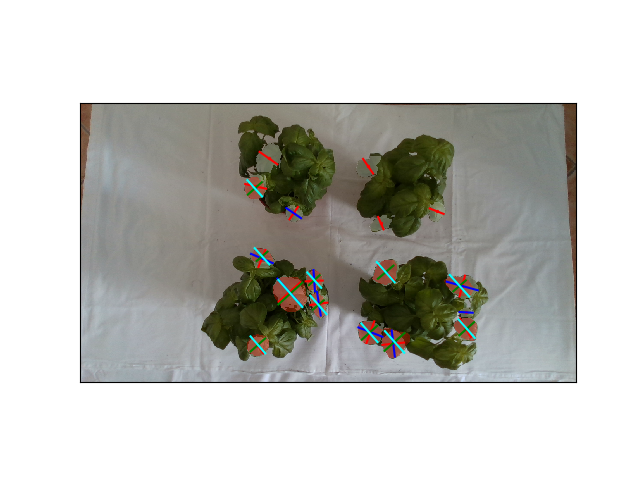
\includegraphics[width=.8\linewidth]{measurement.png}
  \caption{Representation of masks ground truth with correspondent computed one}
\end{figure}

As we can see from the results obtained the net and the measures are relatively accurate as long as the leaf is as linear as possible, unlike in cases where
the leaves are very bent by the weight, our method can not predict these flaws and then the measures are distorted. We can therefore deduce that our method is able
to calculate on average with a good probability the correct size of the leaves with an error of about 5/6 cm.


\begin{figure}[ht] 
  \centering
  \begin{subfigure}{.5\textwidth}
    \centering
    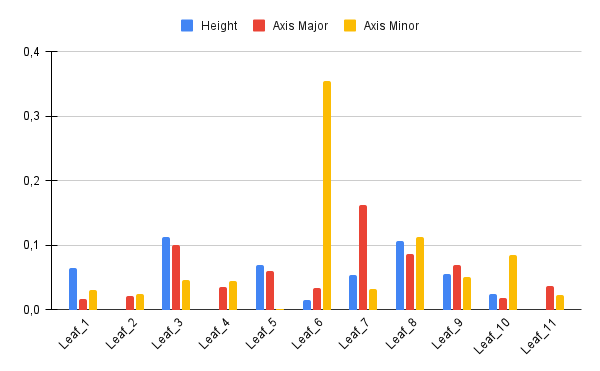
\includegraphics[width=.9\linewidth]{leaf_error}
    \caption{Errors for each measurement}
  \end{subfigure}%
  \begin{subfigure}{.5\textwidth}
    \centering
    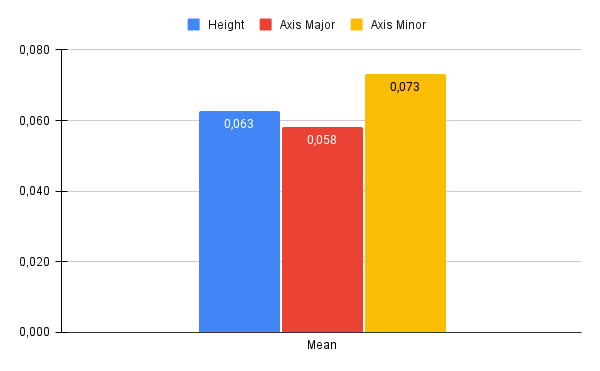
\includegraphics[width=.9\linewidth]{mean_error}
    \caption{Mean error of each measure}
  \end{subfigure}
  \caption{Errors computed from ground truth}
\end{figure}



